
\chapter{Introducción}
\label{cap:introduccion}

\section{Objeto y alcance del trabajo}
\label{sec:objeto_alcance}

\lettrine[lines=3, lhang=0.1]{E}{l} objeto principal de este Trabajo de Fin de Grado (TFG) consiste en el estudio crítico y comparativo de las narrativas técnicas, regulatorias y operativas formuladas por los distintos actores del sector eléctrico, a partir de la información y los informes publicados en respuesta al evento de \textit{Cero de Tensión}\footnote{A lo largo de este documento, los conceptos técnicos específicos resaltados en \textit{cursiva} se encuentran definidos detalladamente en el Glosario Técnico (véase el Anexo \ref{app:glosario}).} (\textit{blackout}) acaecido en el sistema síncrono ibérico el 28 de abril de 2025. Dicho suceso implicó la pérdida súbita de más de 15~GW de generación en apenas unos segundos y dejó sin suministro eléctrico a cerca de 60~millones de personas, constituyendo uno de los episodios de inestabilidad sistémica de mayor magnitud registrados en Europa continental en las últimas décadas \cite{entsoe2025, mitceepr2025}.

\medskip

La naturaleza excepcional del colapso ---caracterizado por una cascada de desconexiones asociadas a fenómenos de sobretensión en un contexto de elevada penetración de \textit{Recursos Basados en Inversores} (\textit{Inverter-Based Resources, IBR})--- ha generado un profundo desacuerdo interpretativo respecto a sus causas raíz y a la asignación de responsabilidades técnicas y operativas. En consecuencia, la presente investigación se aparta de una mera reconstrucción cronológica del evento para centrarse en el examen crítico de las divergencias y puntos de consenso existentes entre las tres visiones institucionales predominantes:

\begin{description}

    \item[Visión de la Administración (Gobierno y Redeia):]
    El informe del Comité de Análisis del Consejo de Seguridad Nacional y del Operador del Sistema (OS) articula una interpretación fundamentada en el cumplimiento normativo y la disciplina técnica del parque generador. Según esta perspectiva, el sistema disponía de herramientas regulatorias suficientes para mitigar el transitorio, atribuyendo el agravamiento del evento a la insuficiente absorción de potencia reactiva inductiva ---un déficit que impidió contener la escalada de tensión--- conforme a los requerimientos establecidos en el Procedimiento de Operación P.O. 7.4 \cite{gobierno2025, ree2025}.

    \item[Visión del Sector Generador (Informe ICAI / AELEC):]
    El informe pericial independiente elaborado por el IIT-ICAI y Compass Lexecon sitúa la causa raíz en decisiones operativas concretas adoptadas por el Operador del Sistema. Esta narrativa cuestiona la maniobra de mallado (\textit{meshing}) ejecutada por Redeia, argumentando que incrementó de forma significativa la contribución capacitiva de la red en un escenario de baja fortaleza síncrona, generando un pulso de sobretensión agravado por las limitaciones de observabilidad del operador sobre la red de 220~kV (fenómeno denominado \textit{Tap-Lag}) \cite{icai2025}.

    \item[Visión del Gestor Europeo (ENTSO-E):]
    El informe factual publicado por ENTSO-E introduce una perspectiva orientada a la estabilidad del área síncrona continental, analizando la propagación de oscilaciones inter-área y señalando las limitaciones de los enfoques tradicionales de seguridad estática basados en el \textit{Criterio $N-1$} frente a fenómenos dinámicos ultrarrápidos propios de sistemas con alta penetración de generación basada en electrónica de potencia \cite{entsoe2025}.

\end{description}

\vspace{0.6cm}
\begin{figure}[H]
    \centering
    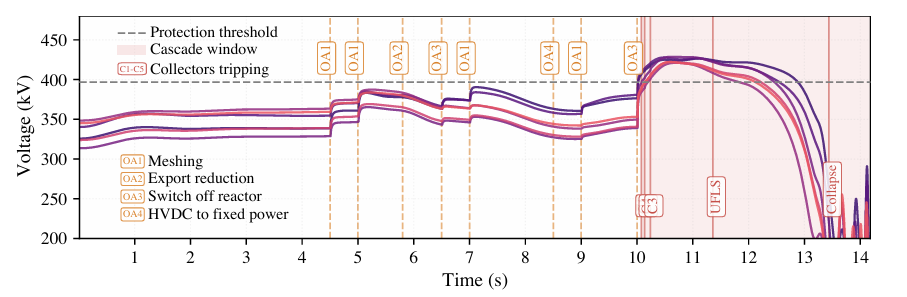
\includegraphics[width=0.65\textwidth]{figuras/albustami_ieee39_secuencia.png}
    \vspace{0.2cm}
    \caption[Replicación de la secuencia del colapso e interacción de acciones OA/AA.]{Replicación de la secuencia del colapso destacando la interacción entre las Acciones del Operador (OA) y las Acciones Automáticas de protección (AA). Fuente: \citeauthor{albustami2025} (\citeyear{albustami2025})}
    \label{fig:albustami_ieee39}
\end{figure}
\vspace{0.6cm}

El alcance del presente TFG se circunscribe al escrutinio técnico de estos marcos argumentales mediante su contraste con los códigos de red europeos (\textit{Network Codes}, especialmente el Reglamento RfG) y con los principios modernos de estabilidad en sistemas eléctricos dominados por inversores. El propósito final es identificar las lecciones estructurales, limitaciones metodológicas y vacíos regulatorios que condicionan la resiliencia del sistema eléctrico europeo durante su transición hacia un modelo energético plenamente descarbonizado.

% --- SECCIÓN 1.2 ---
\section{Justificación técnica: La vulnerabilidad del sistema ibérico frente a la descarbonización}
\label{sec:justificacion_tecnica}

La transición hacia un modelo de generación descarbonizado ha transformado de forma estructural la dinámica del sistema peninsular. La sustitución acelerada de centrales síncronas convencionales por Recursos Basados en Inversores (IBR) reduce las masas rotatorias acopladas a la red y, con ellas, tanto la \textit{inercia del sistema} ($H$) ---que cayó a valores zonales de entre 1,3~s y 1,8~s en el sur peninsular, por debajo del umbral de 2~s que la literatura técnica del sector asocia con márgenes dinámicos comprometidos--- como la \textit{potencia de cortocircuito} disponible en los nudos. Esta doble merma no afecta únicamente al eje frecuencia--potencia activa: debilita también, y de forma crítica, la capacidad del sistema para absorber dinámicamente potencia reactiva ($Q$) y sostener la tensión ante transitorios rápidos, que es precisamente el eje sobre el que se articuló el colapso del 28 de abril \cite{mitceepr2025, futured2024}.

\medskip

Esta vulnerabilidad estructural se manifestó de forma extrema el 28 de abril de 2025. La mañana del incidente, el sistema operaba con un 82~\% de penetración renovable no síncrona, en un contexto de \textit{demanda valle} que redujo la carga en los pasillos de transporte y exacerbó el efecto capacitivo de las líneas de 400~kV. Para equilibrar la generación, el operador desacopló la práctica totalidad de los grupos térmicos disponibles, dejando el número de generadores síncronos en mínimos históricos \cite{blackswan2025, icai2025}.

\vspace{0.5cm}
\begin{figure}[H]
    \centering
    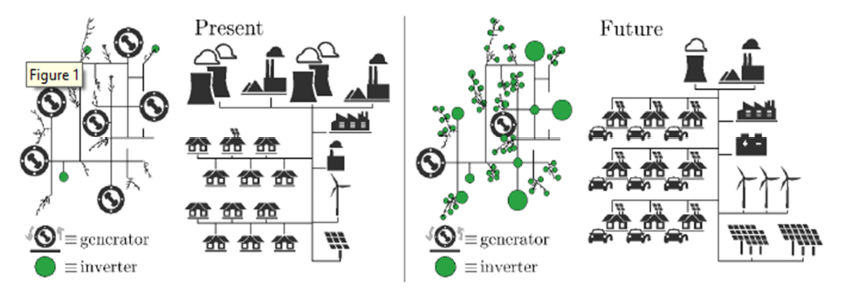
\includegraphics[width=0.75\textwidth]{figuras/futured_grid_evolution.png}
    \vspace{0.2cm}
    \caption[Metamorfosis electromecánica del sistema: de generación síncrona a recursos IBR.]{%
    Metamorfosis electromecánica del sistema de potencia: el desplazamiento
    de grandes masas rotatorias por recursos IBR disminuye drásticamente la
    inercia total. Fuente: \citeauthor{futured2024}}
    \label{fig:futured_metamorfosis}
\end{figure}
\vspace{0.5cm}

Operar bajo este paradigma de ``red ligera'' contrae los márgenes de estabilidad de forma no lineal. A diferencia de los alternadores síncronos, el parque IBR funciona prácticamente en su totalidad en modo \textit{grid-following}: sus inversores necesitan una tensión ($V$) y una frecuencia ($f$) externas estables como referencia de sincronismo. Al reducirse drásticamente los grupos síncronos, el sistema perdió su principal mecanismo de absorción dinámica de potencia reactiva ($Q$), eliminando el amortiguamiento natural frente a transitorios de tensión \cite{futured2024, ree2025}.

\medskip

A esta fragilidad interna se añade la condición estructural de la Península Ibérica como \textit{isla energética}: su capacidad de interconexión con Francia se sitúa muy por debajo de las directrices comunitarias, lo que impide importar estabilidad dinámica desde el núcleo continental. La convergencia de ambos factores ---baja fortaleza síncrona y aislamiento relativo de la red--- configuró la vulnerabilidad que hizo imposible frenar la cascada de sobretensiones a las 12:33:24~CEST \cite{mitceepr2025, icai2025}.

\vspace{0.6cm}
\begin{table}[H]
    \centering
    \caption[Nivel de interconexión eléctrica nominal frente a demanda punta en 2030.]{Nivel de interconexión eléctrica nominal frente a la demanda punta por Estado Miembro (7,9~\% en Iberia). Fuente: MIT CEEPR / Comisión Europea \cite{mitceepr2025}.}
    \vspace{0.3cm}
    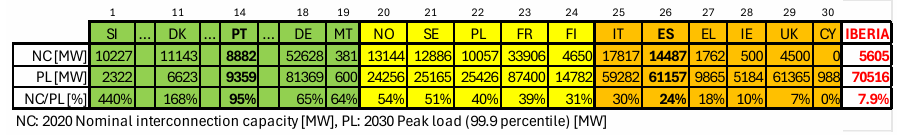
\includegraphics[width=0.8\textwidth]{figuras/mit_interconnection_stats.png}
    \label{tab:mit_interconnection}
\end{table}
\vspace{0.6cm}

% --- SECCIÓN 1.3 ---
\section{Metodología de investigación: Triangulación y análisis asistido por IA}
\label{sec:metodologia}

La metodología de esta investigación se basa en un análisis forense comparativo orientado a reconstruir la secuencia de eventos del 28 de abril de 2025 mediante la triangulación de fuentes primarias divergentes \cite{entsoe2025, gobierno2025, icai2025}. El proceso se ha articulado en tres fases metodológicas:

\begin{enumerate}
    \item \textbf{Compilación de fuentes primarias:} Estudio sistemático de los informes periciales oficiales, que a su vez se sustentan en el procesamiento de más de 170~GB de registros técnicos por parte del Operador del Sistema, incluyendo telemedidas del SCADA y registros oscilográficos \cite{ree2025}.

    \item \textbf{Triangulación de narrativas:} Contraste sistemático de la tesis de la Administración frente al análisis pericial del sector generador en torno a la gestión del mallado y la inobservabilidad de la red de 220~kV \cite{gobierno2025, icai2025}.

    \item \textbf{Validación técnica cruzada:} Cotejo de las secuencias cronológicas de cada informe con el análisis independiente de las oscilaciones inter-área publicado por el NREL a partir de datos de Unidades de Medición Fasorial (PMU), cuya cobertura continental permite arbitrar entre versiones divergentes \cite{nrel2025}.
\end{enumerate}

\vspace{0.6cm}
\begin{figure}[H]
    \centering
    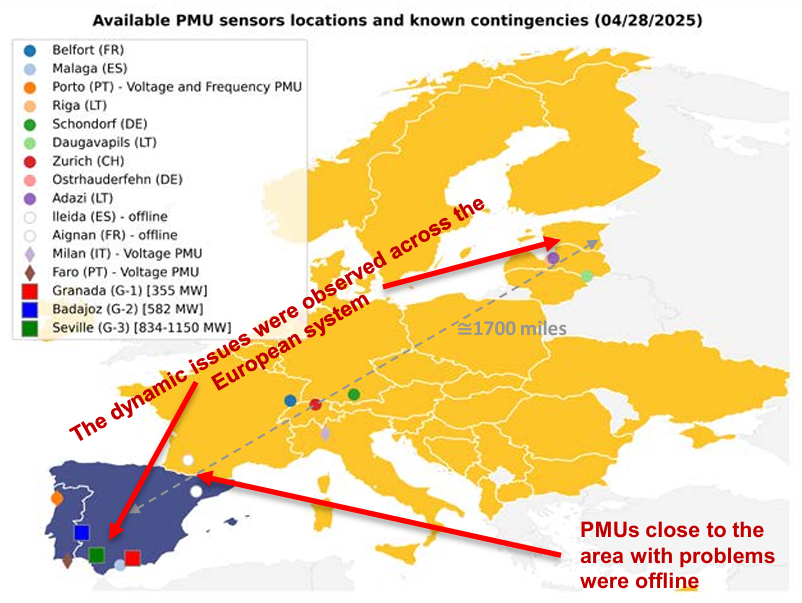
\includegraphics[width=0.65\textwidth]{figuras/pmu_sensors_europe.png}
    \vspace{0.2cm}
    \caption[Localización topológica de las Unidades de Medición Fasorial (PMU) en Europa.]{Localización topológica de las Unidades de Medición Fasorial (PMU) en el sistema síncrono europeo. La captura de datos resultó vital para la verificación de las oscilaciones inter-área. Fuente: NREL / Datos PMU}
    \label{fig:pmu_locations}
\end{figure}
\vspace{0.6cm}

Dado el volumen de documentación técnica generada tras el incidente, se han empleado modelos de lenguaje de gran escala como herramienta de asistencia documental. Su aplicación se ha centrado en la clasificación y síntesis de informes, la extracción de datos críticos y la identificación de patrones de fallo recurrentes entre las distintas fuentes.

\medskip

No obstante, el uso de estas herramientas se ha circunscrito estrictamente a la organización y síntesis documental. Los modelos de lenguaje presentan limitaciones conocidas ante fenómenos de dinámica rápida ---como la interpretación de la paradoja del UFLS o el mecanismo del \textit{Tap-Lag}---, por lo que la comparación técnica, la evaluación de causalidad y las conclusiones del trabajo son responsabilidad exclusiva del criterio del autor.